Pauli matrices:
\[\underbrace{\sigma_z = \Pm{1 & 0\\0 & -1},\;\sigma_x = \Pm{0 & 1\\1 & 0},\;\sigma_y = \Pm{0 & -i\\i & 0}}_{\text{Irreducible representations for Pauli matrices}}\]

This choice is of course not unique but determined by the choice of representation for $\ket{\up}$ and $\ket{\down}$. The basis is irreducible. The set of Pauli matrices is an
irreducible representation for $SU(2)$.
\[
  \begin{array}{ll}
  \left.
  \begin{aligned}
	\Crea_\up\Anni_\up &= \frac{1}{2}\left( 1+\sigma_z \right)\\
	\Crea_\down\Anni_\down &= \frac{1}{2}\left( 1-\sigma_z \right)\\
	\Crea_\up\Anni_\down &= \frac{1}{2}\left( \sigma_x + i\sigma_y \right) = \frac{1}{2}\sigma^+\\
	\Crea_\down\Anni_\up &= \frac{1}{2}\left( \sigma_x - i\sigma_y \right) = \frac{1}{2}\sigma^-
  \end{aligned}
\right\}&\text{\parbox{6cm}{\underline{Note!!} This connection is independent of the representation of the Pauli matrices.}}
\end{array}
\]
Inserting this we get
\[\boxed{\Sum_{\sigma\sigma'}\Crea_{i,\sigma}\Anni_{i,\sigma'}\Crea_{j,\sigma'}\Anni_{j,\sigma} = \frac{1}{2}\left( 1+\gv{\sigma}_i\cdot\gv{\sigma}_j \right).}\]
This can now be regarded as an operator, independent of what representation  is used.
\[\gv{\sigma} = \sigma_x\hat{x} + \sigma_y\hat{y} + \sigma_z\hat{z}.\]
The first term $(\v{T})$ is an uninteresting constant.

\underline{Thus we get in the end:}
\[\Ha = \frac{2t^2}{u}\Sum_{\langle i,j\rangle}\v{S}_i\cdot\v{S}_j = -J\Sum_{\langle i,j\rangle}\v{S}_i\cdot\v{S}_j,\]
where we have defined $\v{S} = 1/2\gv{\sigma}$ and $J = -2t^2/u$, i.e. an antiferromagnetic coupling. Exchange:
\begin{figure}[H]
	\centering
	\begin{tikzpicture}[scale=5,>=stealth',node distance=0.15\textwidth]
	  \node[label={[label distance=4pt]90:$-\frac{1}{u}$}] (n1) {};
	  \node[label={[label distance=4pt]90:$-\frac{t^2}{u}$}] (n2) [right of=n1] {};
		\path[->,thick] (n1.south) edge[bend right=20] node[below=0.3\baselineskip]{$t$} (n2.south);
		\path[->,thick] (n2.north) edge[bend right=20] node[above=0.3\baselineskip]{$t$} (n1.north);
	\end{tikzpicture}
\end{figure}
\begin{Indentskip}
  \underline{Thus:} With one electron pr. lattice site and $u/t\ll 1$, the Hubbard model described an anti-ferromagnetic insulator! It is an insulator because the spins are ``stuck'' on
  the lattice sites and there are no free fermions in the model that can facilitate transport of charge and thus give metallic properties.
\end{Indentskip}
We now give a simple qualitative argument for why we get antiferromagnetism in this model when the band is half-filled.

The hopping term introduces kinetic energy in the problem. What the kinetic energy operator tries to do is to de-localize the electron as much as possible, i.e. it smooths out
the wave function as much as possible. (Remember $K=-\hbar^2\nabla^2\psi/(2m)$, hence kinetic energy wins by reducing the curvature of $\psi$).
What $\Ha_\text{hop}$ does, is it reduces the system's total energy by accessing kinetic energy by delocalize the electron such that we get virtually excited double-occupied states.
\[
\begin{aligned}
  \text{Start} :&\quad\ket{\up,\;\down,\;\up,\;\down,\;\down,\;\phantom{\down}\up,\;\dotsc}\\
  \Ha_\text{hop} :&\quad\ket{\up,\;\down,\;\up,\;\down,\;.\,,\;\,\,\down\up,\;\dotsc}\\
  \Ha_\text{hop} :&\quad\ket{\up,\;\down,\;\up,\;\down,\;\down,\;\phantom{\down}\up,\;\dotsc} = \text{End} = \text{Start}
\end{aligned}
\]
The energy won by this virtual process is then
\[\boxed{\delta E = -\frac{t^2}{u}}\]
\underline{Note}!: The spins on the exchange sites must have opposite spins to access the virtual double-occupied state and thus win energy. It is of course beneficial if
\underline{all} the spins in the system can contribute with $\delta E = -t^2/u$, but then the nearest neighbour spins has to be opposite $\;\Rightarrow\;$
\begin{Indentskip}
  Antiferromagnetic correction!
\end{Indentskip}

We will now return to the more general fermion model and see how it behaves when the band is half-filled. We then consider the matrix-element
$\bra{i_1\;i_2}V\ket{i_3 i_4}$, but now with the $i$s \underline{pairwise} equal. Do such terms lead to spin models? There are three possibilities
\[\left.
  \begin{array}{l@{\quad\quad}l@{\quad}l}
	i) & i_1=i_2\;; & i_3=i_4\\
	ii) & i_1=i_4\;; & i_2=i_3\\
	iii) & i_1=i_3\;; & i_2=i_4
  \end{array}
\right\}\;\text{\parbox{6cm}{Two-center integral with pairwise equal lattice indexes.}}
\]
Remember: Hubbard $\;\Rightarrow\;$ antiferromagnetic model. Can we get a ferromagnetic model with pairwise equal indexes?
\begin{description}
  \item[$i)\phantom{ii}\quad\quad i_1=i_2\;;\quad i_3=i_4\;\quad i_1\neq i_3$]\hfill \\
\[\Sum_{\substack{i_1i_3\\\sigma_1\sigma_2}}\bra{i_1\;i_1}V\ket{i_3\;i_3}\underbrace{\Crea_{i_1\sigma_1}\Crea_{i_1\sigma_2}}_{\sigma_2 = -\sigma_1}
\Anni_{i_3\sigma_2}\Anni_{i_3\sigma_1}
=\Sum_{ij\sigma}\bra{i\;i}V\ket{j\;j}\Crea_{i\sigma}\Crea_{i-\sigma}\Anni_{j-\sigma}\Anni_{j\sigma}\]
This describes hopping of pairs as spin-singlet pairs from $j$ to $i$.
\begin{figure}[H]
	\centering
	\begin{tikzpicture}[scale=5,>=stealth',node distance=0.15\textwidth]
	  \node[label={[label distance=4pt]90:$\up\times\down$}] (n1) {};
	  \node[label={[label distance=4pt]90:$\up\times\down$}] (n2) [right of=n1] {};
		\path[->,thick] (n2.north) edge[bend right=20] node[above=0.3\baselineskip]{} (n1.north);
	\end{tikzpicture}
\end{figure}
This does not lead to $\v{S}_i\cdot\v{S}_j$ since the objects that hop are spinless (total $S_z=0$).

\underline{Note}!: The tunnelling of pairs on the lattices is a result of the electrostatic pair-potential in the same way that one-electron tunnelling was a result of a electrostatic
one-particle potential.

\item[$ii)\phantom{i}\quad\quad i_1=i_4\;;\quad i_2=i_3\;\quad i_1\neq\i_2$]\hfill \\
  \[
	\begin{aligned}
	\Sum_{\substack{i_1i_2\\\sigma_1\sigma_2}}\bra{i_1i_2}V\ket{i_2i_1}\Crea_{i_1\sigma_1}\Crea_{i_2\sigma_2}\Anni_{i_2\sigma_2}\Anni_{i_1\sigma_1}
  &= \Sum_{\substack{ij\\\sigma\sigma'}} \bra{ij}V\ket{ji}\Crea_{i\sigma}\Anni_{i\sigma}\Crea_{j\sigma'}\Anni_{j\sigma'}\\
  &= \Sum_{ij}\bra{ij}V\ket{ji}n_in_j.
	\end{aligned}
  \]
  A purely electrostatic interaction between charges. No spin structure. Does \underline{not} result in $\v{S}_i\cdot\v{S}_j$.
\item[$iii)\quad\quad i_1=i_3\;;\quad i_2=i_4\;;\quad i_1\neq i_2$]\hfill \\
  \[
	\begin{aligned}
	  \Sum_{\substack{i_1i_2\\\sigma_1\sigma_2}}\bra{i_1i_2}V\ket{i_1i_2}\Crea_{i_1\sigma_1}\Crea_{i_2\sigma_2}\Anni_{i_1\sigma_2}\Anni_{i_2\sigma_1}
	  &= -\Sum_{\substack{ij\\\sigma\sigma'}}\bra{ij}V\ket{ij}\underbrace{\Crea_{i\sigma}\Anni_{i\sigma'}\Crea_{j\sigma'}\Anni_{j\sigma}}_\text{\parbox{4cm}
	  {This we have encountered before
	  and the result is:}}\\
	  &= -\Sum_{ij}2\bra{ij}V\ket{ij}\v{S}_i\v{S}_j.
	\end{aligned}
  \]
\end{description}

\underline{Note}!: So far we have not used anything about half-filling of the band. By using $i=\cdots i_4$, and $i_1,\cdots,i_4$ pairwise equal we can thus write down a general
model for metals that can be magnetic:

\[
  \begin{aligned}
	&\Ha = \Sum_{ij}t_{ij}\Crea_{i\sigma}\Anni_{j\sigma} + \frac{u}{2}\Sum_{i\sigma}n_{i\sigma}n_{i-\sigma}\\
	\text{\parbox{6cm}{Two-center integrals with pairwise equal lattice indices}} &\left\{
	  \begin{aligned}
		+ & \Sum_{ij}V_{ij}n_in_j + \Sum_{ij\sigma}t_{ij}^P\Crea_{i\sigma}\Crea_{i-\sigma}\Anni_{j-\sigma}\Anni_{j\sigma}\\
		- & \Sum_{ij}\tilde{J}_{ij}\v{S}_i\cdot\v{S}_j\quad\text{\parbox{4cm}{$i,j$: Not necessarily nearest neighbours!}}
	  \end{aligned}
	  \right.
  \end{aligned}
\]

A completely general model would have included correlated hopping which also is a two-particle process. In the above equation we have defined
\[
  \begin{aligned}
	u = \bra{ii}V\ket{ii},\quad&\\
	V_{ij} = \bra{ij}V\ket{ji}\quad&\text{Electrostatic},\\
	t_{ij}^P = \bra{ii}V\ket{jj}\quad&\text{Tunnelling of pairs},\\
	\tilde{J}_{ij} = 2\bra{ij}V\ket{ij}\quad&\text{Spin coupling}.
  \end{aligned}
\]
When we have $1/2$ filling, the two first terms is replaced by a spin model, as we have already seen. The third term is uninteresting when there is not dynamic of the charges in
the problem, as is the 4th term. In that case what remains is
\[\Ha = -\Sum_{ij}\tilde{\tilde{J}}_{ij}\v{S}_i\cdot\v{S}_j\;;\quad\quad\tilde{\tilde{J}}_{ij} = 2\left[ \tilde{J}_{ij} - \frac{t^2}{u} \right].\]
It is clear that $\tilde{\tilde{J}}_{ij}$ can give both ferro- and antiferromagnetism!

\subsection{Heisenberg model}
The model
\[\Ha = -\sum_{ij}J_{ij}\v{S}_i\cdot\v{S}_j\]
is often called the \emph{Heisenberg model}. Here $\v{S}$ are dimensionless spin operators and $J_{ij}$ are given by matrix elements that contains a one-particle or two-particle
potential.

Even though such models has classical counterparts, we see that interaction of spins is quantum mechanical in nature. With the previously introduced spin operators we have
\[ [S_x,\;S_y] = iS_z\quad\text{etc.} \]
by cyclic permutations. It is these non-trivial commutator relations that gives a quantum mechanical spin system. For a classical model the spin operators commute. Because of the
non-trivial commutators we get uncertainty in the determination of the spin components. We get \emph{quantum fluctuations}. We could also have generalized the model a bit:
\[ \Ha = -\Sum_{ij}\left( J_{ij}^\ast S_i^\ast S_j^\ast + (y) + (z) \right).\]
A possibly cause for such anisotropy could be e.g. anisotropic one-particle hopping in the Hubbard model. The Heisenberg model is solved exactly in one dimension 
for a general coupling when $(i,j)$
are limited to nearest neighbours~\cite{bethe1931}.

In two dimensions the classical model with $J^x = J^y = 0$ is solved exactly~\cite{onsager1943}. The two-dimensional quantum mechanical model with isotropic coupling is of great 
interest lately since quantum fluctuations are assumed to be large in $2$D for $S=1/2$. This can result in interesting ``new'' types of ground states, completely different from the
``classical'' ferromagnetic ground states, or antiferromagnetic N\'{e}el states, see e.g.~\cite{charkravarty1989} or~\cite{chubukov1993}.

At Brookhaven National Laboratories and MIT there has recently been initiated large scale experiments to find these new and exotic magnetic ground states
in low-dimensional $S=1/2$ quantum magnets. Finally, let us remark that we started with a \emph{fermion} model, but the effective Hamilton operator at $1/2$-filled lattice
(the Heisenberg model) is not a fermion model (and neither a boson model). The spin operators do not satisfy the fermion (boson) commutation relations.

%% I don't see the point of writing down page 70a) since it didn't make much sense to me.

%Ising: $J^x=J^y=0$. Still quantum mechanical. Model with rotation of the plane ($xy$ model).
%\[J^z = 0\].
%Ising: $\mathbb{Z}_2$-symmetry. Discrete.
%\[xy:\quad O(2)\quad\quad\text{Continuous}\]
%\[\text{Heisenberg}\quad O(3)\quad\quad\text{Continuous}\]
%\[\v{S}_i\cdot\v{S}_j\]

\subsection{Low temperature properties of magnetic insulators}
\paragraph{Generalities}\hspace{0pt}\\
The spin operators ($S=1/2$) have the following properties
\[[S_{ix},\;S_{jy}] = i\delta_{ij}S_{iz},\]
where cyclic permutation of spin components applies. The ladder operators for spin:
\[\begin{array}{r@{\;}c@{\;}l}
	S_i^\pm 					& =	& S_{ix}\pm iS_{iy}\\\\
	S_i^+\ket{\up}=0			& ;	& \quad S_i^+\ket{\down} = \ket{\up}\\\\
	S_i^-\ket{\up}=\ket{\down}	& ;	& \quad S_i^-\ket{\down} = 0\\\\
	\commum{S_{iz},S_j^\pm}		& =	& \pm\delta_{ij}S_j^\pm\\\\
	\commum{S_i^+,S_j^-}		& =	& 2\delta_{ij}S_{iz}
\end{array}\]
The total spin on the complete lattice is given by
\[\v{S}_T=\sum_i\v{S}_i,\qquad\text{where}\qquad S_{Tz} = \Sum_iS_{iz}.\]
Magnetization: $\langle S_{Tz}\rangle = \Sum_i\langle S_{iz}\rangle$, where $\langle\;\cdot\;\rangle$ is the statistical average.

\paragraph{$S_{iz},\;S_i^\pm$} are neither fermion or boson operators. What kind of operators are they? Consider e.g. a ferromagnetic ground state
\[\ket{\psi_0} = \ket{\;\up\;\up\;\up\;\dotsc\;\up}.\]
All the spins point ``upwards''. This is an eigenstate of $S_{iz}$.
\[\underbrace{S_{iz}}_{\text{operator}}\ket{\psi_0} = \underbrace{S_{iz}}_\text{number}\ket{\psi_0}\]
Thus it measures the $z$-component of the spin on lattice site $i$.

\[\begin{array}{r@{\;}c@{\;}l}
	S_i^+\ket{\psi_0}	& =	& 0\\\\
	S_i^-\ket{\psi_0}	& =	& \ket{\;\up\;\up\;\dotsc\;\underbrace{\down}_i\;\dotsc\;\up}.
\end{array}\]
This is a spin flip on lattice site $i$. We obtain energy: $4S^2J$ i.e. the process ($\up\up\;\mapsto\;\up\down$) $\;\Rightarrow\;\Delta E = 2JS^2$.
The commutator relations for $S_z$ and $S^\pm$ show that this excitation neither is a fermion, nor a boson. We shall later see that it is possible to find completely
different excitations with much lower energy and that is far ``smoother'', i.e. they represent less dramatic changes from the ground state.
Our aim is to find a description of these low energy excitations in terms of fermion or boson operators and if possible, such that there are no interactions in the theory, i.e.
such that the theory is ``free''. As it turns out it is possible to find such a description using boson operators. It is emphasized here that this description is most
useful for low energy fluctuations about the ground state of the magnet, i.e. it is only valid at low temperatures. This description also requires that the ground state is
\emph{ordered}. We first consider \underline{ferromagnetism} (closes neighbour):

\[\Ha = -\Sum_{ij}J_{ij}\v{S}_i\cdot\v{S}_j\quad;\quad J_{ij}>0\]

We solve this problem by introducing the \emph{Holstein-Primakoff} transformation for ferromagnets. The Holstein-Primakoff transformation expresses the spin-operators accurately
in terms of boson operators. (bosonization of the spin problem)
\paragraph{H-P}:\hspace{0pt}
\[S_{iz} = S-\Creab_i\Annib_i\;;\quad S\in\mathbb{R} \;\;(=1/2)\]
$\Creab\Annib:$ Number operator that causes spin-fluctuations of the ground state at lattice site $i$. $\Creab_i\Annib$ reduces the max spin component slightly.
The expression for $S_i^\pm$ is a bit more complicated:
\[
  \begin{aligned}
	S_i^+ &= \sqrt{2S}\left( 1-\frac{1}{2S}\Creab_i\Annib_i \right)^{(1/2)}\Annib_i\\
	S_i^- &= \sqrt{2S}\Creab_i\left( 1- \frac{1}{2S}\Creab_i\Annib_i \right)^{(1/2)}
  \end{aligned}
\]
Holstein and Primakoff discovered that if the boson operators $\Annib_i$ satisfies
\[ \left[ \Annib_i,\Creab_j \right] = \delta_{ij},\quad\text{etc.}\]
then $S_{iz}, S_i^\pm$ satisfy the correct spin commutation relations.

\underline{Note}!: The expression $(\hspace{9pt})^{(1/2)}$ is meant to be interpreted as a series expansion in the boson operators.

\begin{Indentskip}
  Exercise: Verify that the spin commutation relations are satisfied
\end{Indentskip}

If we now insert H-P into $\Ha$ we get an equally difficult problem. The problem is then simplified drastically by assuming that the local fluctuations in the ground state are small:
\[\avg{\Creab_i\Annib_i}\;\ll\;S \quad\Rightarrow\]
\[
  \begin{aligned}
	S_i^+ &\simeq \sqrt{2S}\Annib_i + \mathcal{O}(a^3)\\
	S_i^- &\simeq \sqrt{2S}\Creab_i + \mathcal{O}(a^3)
  \end{aligned}
\]
This can be regarded as an expansion in large $S$.
\[S_{iz} = S - \Creab_i\Annib_i\]
\begin{align*}
  \Ha &= -J\Sum_{\avg{i,j}}\;\left( \v{S}_i\cdot\v{S}_j \right)\\
  &= -J\Sum_{\avg{i,j}}\;\left[ S_{iz}S_{jz} + S_i^+S_j^- \right]
\end{align*}
Now we insert the approximations for the $S$ operators and neglect all terms of order $2$ or more in $a\quad\Rightarrow$
\begin{align*}
  \Ha &= -J\Sum_{\avg{i,j}}\left( S^2 - S\Creab_i\Annib_i - S\Creab_j\Annib_j + 2S\Annib_i\Creab_j \right)\\
  &= E_0 + JS\Sum_{\avg{i,j}}\left( \Creab_i\Annib_i + \Creab_j\Annib_j - 2\Annib_i\Creab_j \right)
\end{align*}
where we have defined $E_0 = -J\Sum_{\avg{i,j}}S^2 = -JS^2Nz$ for $N = $ \emph{number of lattice sites} and $z = $ \emph{number of nearest neighbours}.

Since we have $i\neq j$ in the sum we know $\Annib_i\Creab_j = \Creab_j\Annib_i$, thus we can write
\[\Ha = E_0 + 2JS\Sum_{\avg{i,j}}\left( \Creab_i\Annib_i - \Creab_i\Annib_j \right)\]
We wish to write the boson term of the form
\[\Sum_\lambda\omega_\lambda\underbrace{\Creab_\lambda\Annib_\lambda}_\text{\parbox{2cm}{Same quantum number}}\;: \quad\quad\text{Free boson gas}\]

$\omega_\lambda$: Excitation energy of the bosons (spin fluctuations) in the problem. We achieve such a ``diagonalization'' by introducing the Fourier transformed operators
\begin{align*}
  \Annib_\v{q}&=\frac{1}{\sqrt{N}}\Sum_j \Annib_je^{i\v{q}\cdot\v{r}_j}\\
  \Creab_\v{q}&=\frac{1}{\sqrt{N}} \Sum_j \Creab_je^{-i\v{q}\cdot\v{r}_j}
\end{align*}
where $\v{q}$ runs over the first Brillouin zone of the reciprocal lattice. Then
\begin{align*}
  \Sum_i\Creab_i\Annib_i &= \Sum_q\Creab_q\Annib_q\quad\Rightarrow\\
  \Sum_{\avg{i,j}}\Creab_i\Annib_i &= z\Sum_\v{q}\Creab_q\Annib_q.
\end{align*}
\[\Sum_{\avg{i,j}} \Creab_i\Annib_j = \frac{1}{N}\Sum_{\avg{i,j}}\Sum_{q_1q_2}\Creab_{q_1}\Annib_{q_2}e^{i(\v{q}_2\cdot\v{r}_j - \v{q}_1\cdot\v{r}_i)}.\]
If we now define $\gv{\delta}$ by
\[\v{r}_j = \v{r}_j + \gv{\delta}\]
then $\gv{\delta}$ is the vector from $\v{r}_i$ to nearest neighbour and we can write
\begin{align*}
  \Sum_i\Creab_i\Annib_i &= \frac{1}{N}\Sum_i\Sum_{\gv{\delta}}\Sum_{q_1q_2}\Creab_{q_1}\Annib_{q_2}e^{-i(\v{q}_1 - \v{q}_2)\cdot\v{r}_i}e^{i\v{q}_2\cdot\gv{\delta}}\\
  &= \Sum_{\v{q}_1}\Sum_{\gv{\delta}}\Creab_{q_1}\Creab_{q_2}e^{i\v{q}_1\cdot\gv{\delta}}.
\end{align*}
Inserting this into $\Ha$ we get
\begin{Indentskip}
\begin{align*}
  \Ha &= E_0 + 2JS\Sum_{\v{q}}\left\{\Sum_{\gv{\delta}}\left( 1-e^{i\v{q}\cdot\gv{\delta}} \right)\right\}\Creab_q\Annib_q\\
  &= E_0 + \Sum_\v{q}\omega_q\Creab_q\Annib_q.
\end{align*}
\[\omega_{\B{q}} = 2JS\Sum_{\gv{\delta}}\left( 1-e^{i\v{q}\cdot\gv{\delta}} \right)\]
\end{Indentskip}



\subsection{2D quadratic lattice}
In the 
\[\omega_{\B{q}}=2JS\big(4-2\cos(q_xa)-2\cos(q_ya)\big),\]
where $a$ is the lattice constant. In the case of small $\B{q}$ we get
\[\begin{array}{r@{\;}c@{\;}l}
	\omega_{\B{q}}	& \approx	& 2JS\left[4-2\left(1-\dfrac{(q_xa)^2}{2}\right)-2\left(1-\dfrac{(q_ya)^2}{2}\right)\right]\\\\
					& =			& 2JS\B{q}^2a^2,\\\\
	\B{q}^2			& =			& q_x^2+q_y^2.
\end{array}\]
This behaviour is shown in figure~\ref{fig:omega_quadratic}. In other words: those fluctuations that we have found, have an excitation energy that depends quadratically on the wave number of the fluctuations, when they have long wavelengths. Compare
\[\omega_{\B{q}}\approx2JS\B{q}^2a^2\]
with
\[\Delta E=4JS^2\]
for a local spin flip with
\[\omega_{\B{q}}\ll\Delta E,\qquad |\B{q}|a\ll 1.\]

\begin{figure}
	\centering
	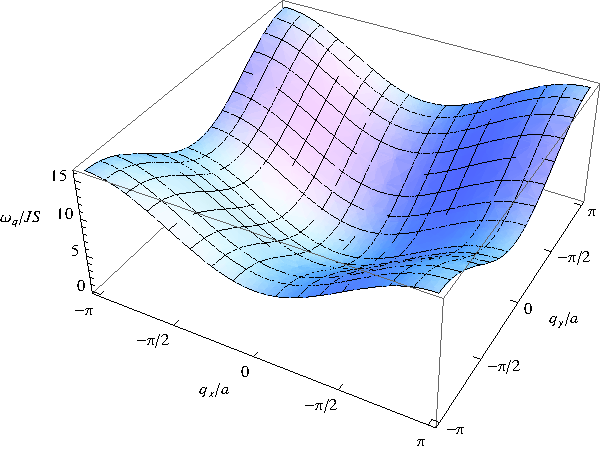
\includegraphics{img/omega_quadratic_compress}
	\caption{\label{fig:omega_quadratic_compress}The angular frequency $\omega_{\B{q}}$ as a function of the momentum $\B{q}$.}
\end{figure}

The fluctuations we have found are spin waves, as is shown in figure~\ref{fig:spin_wave}. The operators $\Creab_{\B{q}}$ and $\Annib_{\B{q}}$ are the creation and annihilation operators for the quantized excitations of these waves. The quantized spin waves are called \Underline{magnons}. These are bosons, because they are described by boson operators.
\begin{figure}
	\centering
	\begin{tikzpicture}[>=stealth',scale=2]
		\draw[->,dashed] (0,1)--(0,2);
		\draw[->] (0,1)--(0.3,1.924);
		\draw[dashed] (0,1.924) ellipse (0.3cm and 0.05cm);
		\draw[->,dashed] (1,1)--(1,2);
		\draw[->] (1,1)--(1,1.974);
		\draw[dashed] (1,1.924) ellipse (0.3cm and 0.05cm);
		\draw[->,dashed] (2,1)--(2,2);
		\draw[->] (2,1)--(1.7,1.924);
		\draw[dashed] (2,1.924) ellipse (0.3cm and 0.05cm);
		\draw[->,dashed] (3,1)--(3,2);
		\draw[->] (3,1)--(3,1.874);
		\draw[dashed] (3,1.924) ellipse (0.3cm and 0.05cm);
		\draw[->,dashed] (4,1)--(4,2);
		\draw[->] (4,1)--(4.3,1.924);
		\draw[dashed] (4,1.924) ellipse (0.3cm and 0.05cm);
		\draw[thick] (0,0) sin (1,0.3) cos (2,0) sin (3,-0.3) cos (4,0);
		\draw[->] (0,0)--(0.3,0);
		\draw[dashed] (0,0) circle (0.3cm);
		\draw[->] (1,0)--(1,0.3);
		\draw[dashed] (1,0) circle (0.3cm);
		\draw[->] (2,0)--(1.7,0);
		\draw[dashed] (2,0) circle (0.3cm);
		\draw[->] (3,0)--(3,-0.3);
		\draw[dashed] (3,0) circle (0.3cm);
		\draw[->] (4,0)--(4.3,0);
		\draw[dashed] (4,0) circle (0.3cm);
	\end{tikzpicture}
	\caption{\label{fig:spin_wave}The spins precess slowly in space, creating spin waves.}
\end{figure}

The effective low-energy Hamiltonian for the spin model,
\[\Ha=-J\Sum_{\braket{i,j}}\B{S}_i\cdot\B{S}_j,\qquad J>0,\]
is thus given by a free boson theory:
\[\Ha=\Sum_{\B{q}}\omega_{\B{q}}\Creab_{\B{q}}\Annib_{\B{q}}.\]
We have a \Underline{lattice fermion} model with half-filled bands in the strongly correlated case. This was found to describe a ferromagnetic insulator (we chose to look at it in the ferromagnetic case). This gave rise to a free \Underline{boson theory} for ferromagnetic bosons (magnons)! 
%Not sure if this should be included
For the ferromagnetic case, see the exercise.

The magnetization of ferromagnets at $T>0$:
\[\Ha=\Sum_i\Braket{S-\Creab_i\Annib_i}=NS-\Sum_{\B{q}}\Braket{\Creab_{\B{q}}\Annib_{\B{q}}}.\]
Using that
\[\Ha=\Sum_{\B{q}}\omega_{\B{q}}\Braket{\Creab_{\B{q}}\Anni_{\B{q}}},\qquad \Braket{\Creab_{\B{q}}\Annib_{\B{q}}}=\dfrac{1}{e^{\beta\omega_{\B{q}}}-1},\]
(assuming a Bose distribution)
\[\Ha=NS-N\Int\dfrac{d^dq}{(2\pi)^d}\,\dfrac{1}{e^{BJS\B{q}^2}-1}.\]
For low temperatures $T$, where $\beta\gg\omega_{\B{q}}$, only small $\B{q}$ will contribute!